\subsection{Components}

\note{Feel free to move and change the name of this subsection later}

\insertbigimage{figures/block_diagram.pdf}{Block diagram of the system}{block_diagram}

As seen in \cref{block_diagram} there were lots of blocks


\textbf{Sensors}

SDI-12

\begin{figure}
    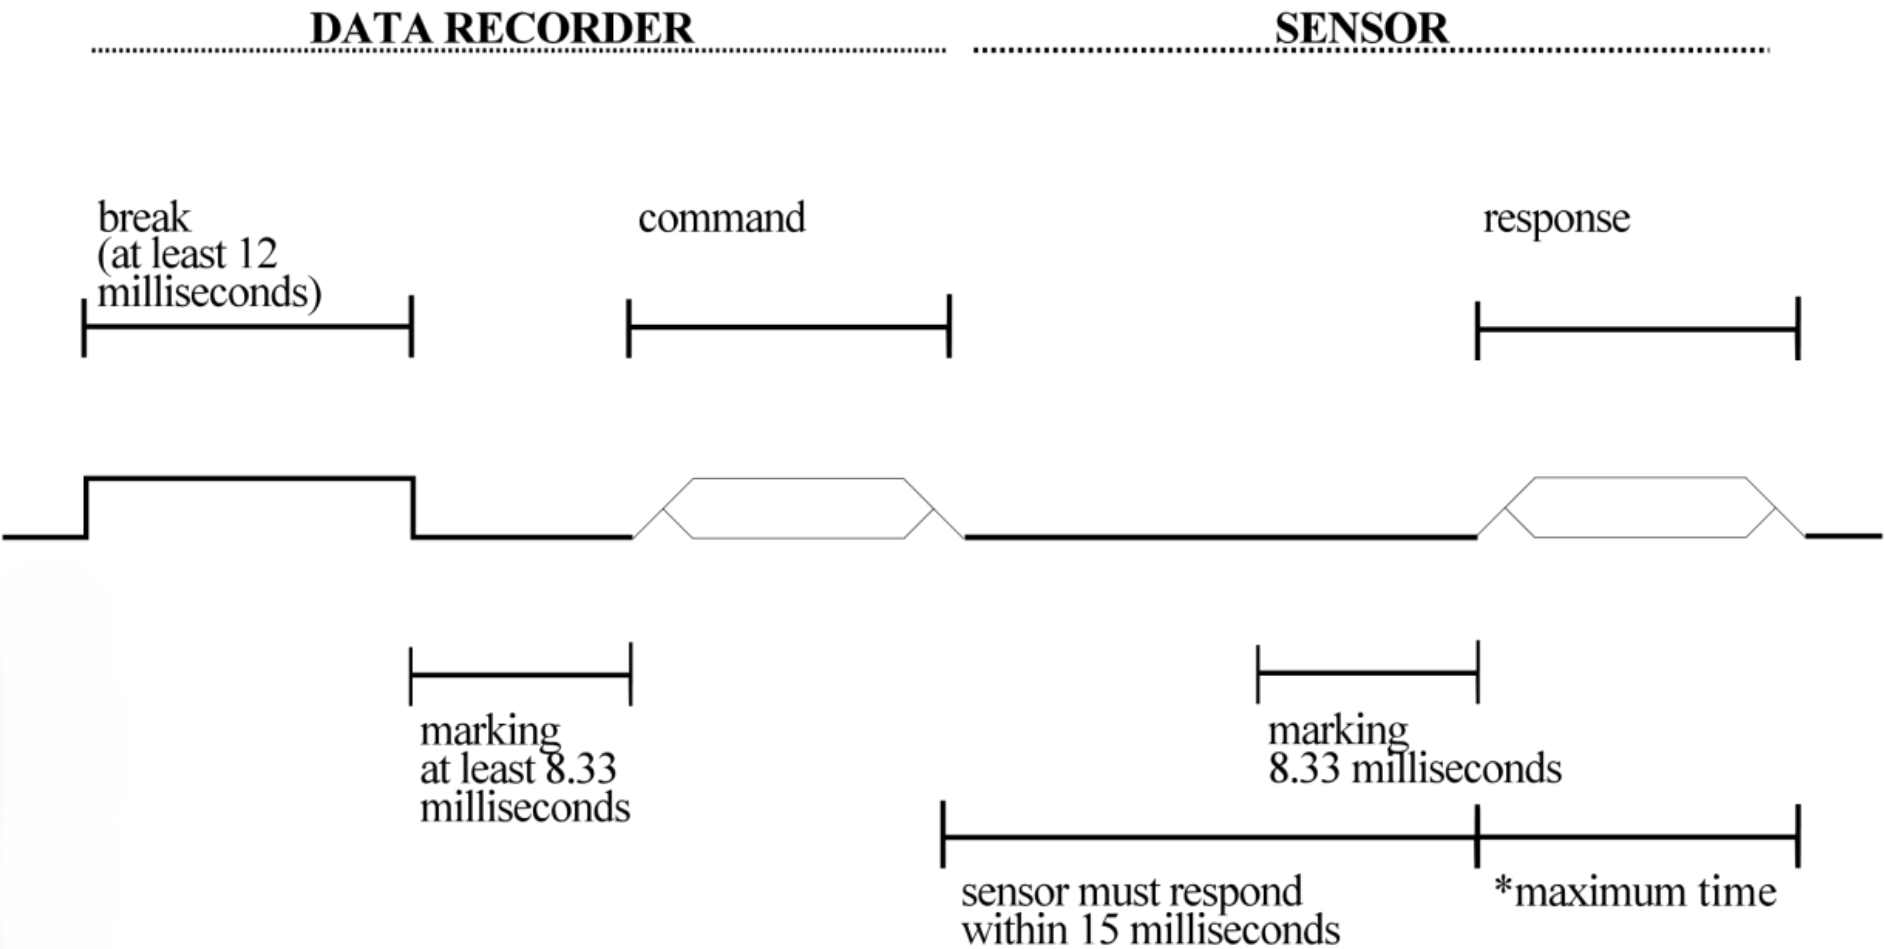
\includegraphics[width=\linewidth]{figures/SDI-12_timing.png}
    \caption{SDI-12 timing from \cite{sdi12_datasheet}}
    \label{sdi12_timing}
\end{figure}

we used the \code{uart_break()} function to send the break signal, and then used the \code{uart_read_stuff()} function to read the response from the sensor. The response was then parsed to get the data. The timing of the SDI-12 protocol is shown in \cref{sdi12_timing}.

Load Cell (MT603)
analogue signal, therefore requires ADC?

Sap Flow Sensor (SF5)
uses SDI-12

Leaf thermistor
uses SDI-12

\textbf{Things to check:}
\begin{itemize}
    \item is 12V necessary?
    \item should we choose I2C or SPI (or both) as interface between RP2040 and DAC?
    \item do we want bluetooth or wifi?
\end{itemize}
- crystal like in assignment 1?
- ADC for load cell?